\documentclass[12pt,a4paper]{report}

\usepackage{tikz}
\usetikzlibrary{matrix,chains,positioning,decorations.pathreplacing,arrows, automata}
\begin{document}


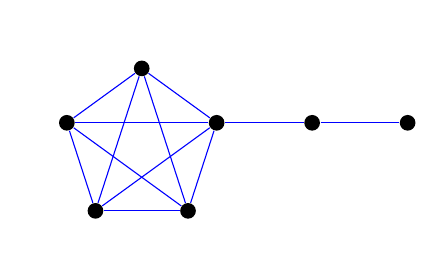
\begin{tikzpicture}[bullet/.style={circle, fill, inner sep=2pt}]
    \foreach \lab [count=\c, 
                   evaluate=\c as \ang using {18+72*\c}] 
    in {a, b, c, d, e} {
       \node[bullet] (\c) at (\ang:10mm) {};
       \node at (\ang:14mm){};
       \foreach \i in {1,...,\c} {
          \draw[blue](\i)--(\c);
       }
    }
    
        \node[bullet] (6) [right=of 5] {};
    \node[bullet] (7) [right=of 6] {};
    \draw[blue] (5) -- (6);
    \draw[blue] (6) -- (7);
  \end{tikzpicture}


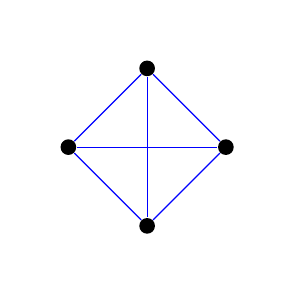
\begin{tikzpicture}[point/.style={circle, fill, inner sep=2pt}]
    \foreach \lab [count=\c, 
                   evaluate=\c as \ang using {90*(\c)}] 
    in {a, b, c, d} {
       \node[point] (\c) at (\ang:10mm) {};
       \node at (\ang:14mm){};
       \foreach \i in {1,...,\c} {
          \draw[blue](\i)--(\c);
       }
    }
   
  \end{tikzpicture}





\end{document}